%% fig03-wrap-clip-mask, caption is in docs/figures/README.md
\documentclass[border=8pt]{standalone}
% Shared preamble for the interpolation-geometry figures.
% \input by every figNN-*.tex. 
\usepackage[T1]{fontenc}
\usepackage{amsmath,amssymb}
\usepackage{tikz}
\usetikzlibrary{shapes.misc,arrows.meta,calc,decorations.pathreplacing,positioning,fit,backgrounds}

\definecolor{ink}{HTML}{1A1A1A}
\definecolor{gridc}{HTML}{9AA3AD}
\definecolor{accent}{HTML}{1F5FA9}
\definecolor{good}{HTML}{2E7D4F}
\definecolor{bad}{HTML}{B03030}
\definecolor{soft}{HTML}{E6EDF7}
\definecolor{softg}{HTML}{E3F0E8}
\definecolor{softr}{HTML}{F8E6E6}
\definecolor{amber}{HTML}{B8860B}


\tikzset{
  gpt/.style={circle,fill=ink,inner sep=1.15pt},
  ghost/.style={circle,draw=gridc,fill=white,inner sep=1.15pt},
  dep/.style={cross out,draw=accent,thick,inner sep=1.6pt,minimum size=4pt},
  traj/.style={gridc,dotted,thick,-{Stealth[length=2mm]}},
  htraj/.style={accent,very thick,-{Stealth[length=2.6mm]}},
  lbl/.style={font=\footnotesize},
  slbl/.style={font=\scriptsize},
}

\begin{document}
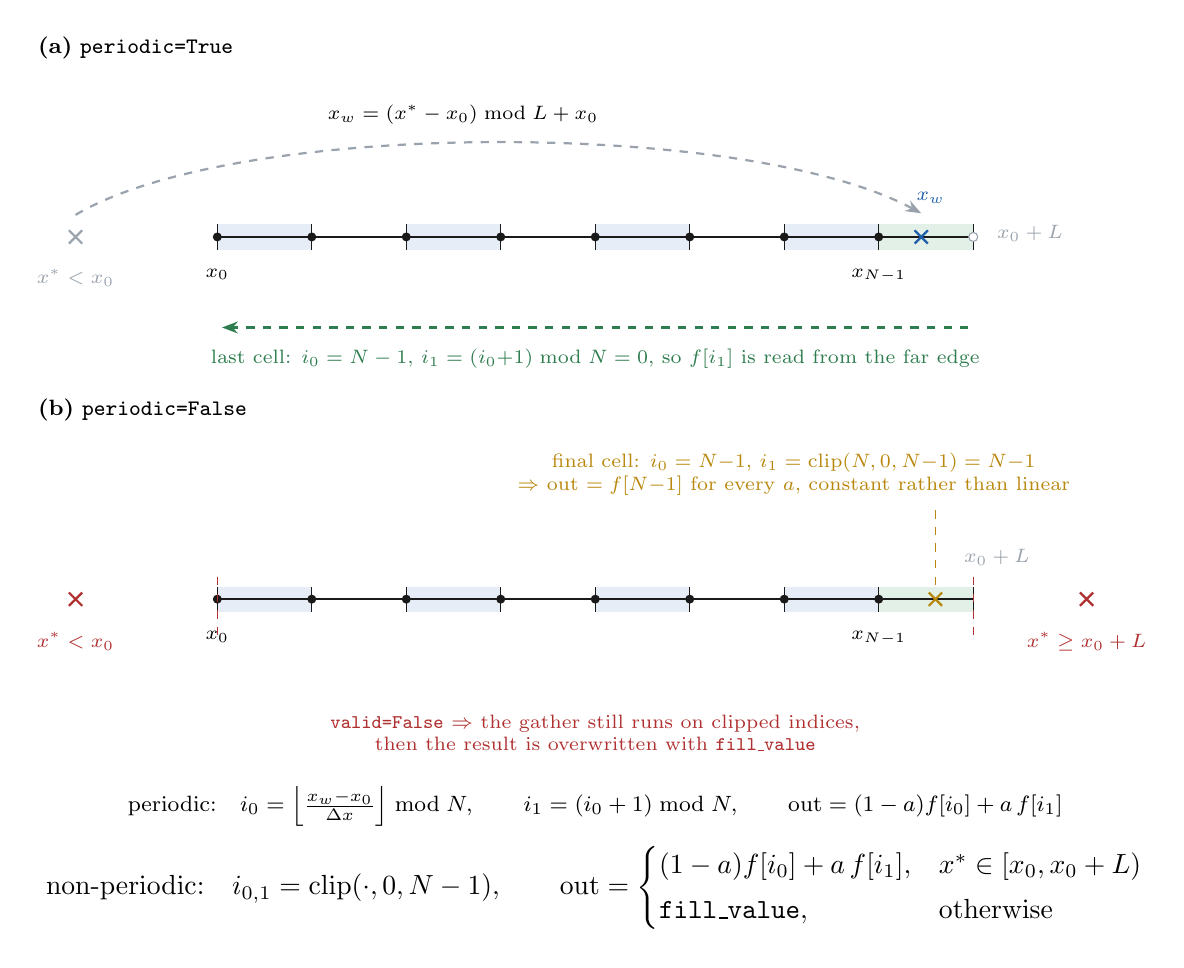
\begin{tikzpicture}[x=1.2cm,y=1cm]
  % ===================== (a) periodic =====================
  \begin{scope}
    \node[lbl,anchor=west] at (-2.0,2.4) {\textbf{(a)} \texttt{periodic=True}};
    \foreach \k in {0,2,4,6} \fill[soft] (\k,-0.16) rectangle (\k+1,0.16);
    \fill[softg] (7,-0.16) rectangle (8,0.16);
    \draw[ink,thick] (0,0) -- (8,0);
    \foreach \i in {0,...,8} \draw[ink] (\i,-0.16) -- (\i,0.16);
    \foreach \i in {0,...,7} \node[gpt] at (\i,0) {};
    \node[ghost] at (8,0) {};
    \node[slbl,anchor=north] at (0,-0.28) {$x_0$};
    \node[slbl,anchor=north] at (7,-0.28) {$x_{N-1}$};
    \node[slbl,anchor=west,gridc] at (8.15,0.05) {$x_0+L$};
    \node[dep,gridc] at (-1.5,0) {};
    \node[slbl,gridc,anchor=north] at (-1.5,-0.28) {$x^{*}<x_0$};
    \draw[gridc,thick,dashed,-{Stealth[length=2mm]}]
       (-1.5,0.28) .. controls (0.2,1.5) and (5.6,1.5) .. (7.45,0.3);
    \node[dep] at (7.45,0) {};
    \node[slbl,accent,anchor=south] at (7.55,0.3) {$x_w$};
    \node[slbl,anchor=south] at (2.6,1.3) {$x_w=(x^{*}-x_0)\bmod L+x_0$};
    \draw[good,dashed,thick,-{Stealth[length=2mm]}] (7.95,-1.15) -- (0.05,-1.15);
    \node[slbl,good,anchor=north] at (4,-1.3)
      {last cell: $i_0=N-1$, $i_1=(i_0{+}1)\bmod N=0$, so $f[i_1]$ is read from the far edge};
  \end{scope}
  % ===================== (b) non-periodic =====================
  \begin{scope}[yshift=-4.6cm]
    \node[lbl,anchor=west] at (-2.0,2.4) {\textbf{(b)} \texttt{periodic=False}};
    \foreach \k in {0,2,4,6} \fill[soft] (\k,-0.16) rectangle (\k+1,0.16);
    \fill[softg] (7,-0.16) rectangle (8,0.16);
    \draw[ink,thick] (0,0) -- (8,0);
    \foreach \i in {0,...,8} \draw[ink] (\i,-0.16) -- (\i,0.16);
    \foreach \i in {0,...,7} \node[gpt] at (\i,0) {};
    \node[slbl,anchor=north] at (0,-0.28) {$x_0$};
    \node[slbl,anchor=north] at (7,-0.28) {$x_{N-1}$};
    \node[slbl,anchor=south,gridc] at (8.25,0.3) {$x_0+L$};
    \draw[bad,dashed] (8,0.28) -- (8,-0.55);
    \draw[bad,dashed] (0,0.28) -- (0,-0.55);
    \node[dep,bad] at (-1.5,0) {};
    \node[dep,bad] at (9.2,0) {};
    \node[slbl,bad,anchor=north] at (-1.5,-0.3) {$x^{*}<x_0$};
    \node[slbl,bad,anchor=north] at (9.2,-0.3) {$x^{*}\ge x_0+L$};
    \node[slbl,bad,anchor=north,align=center] at (4,-1.35)
      {\texttt{valid=False} $\Rightarrow$ the gather still runs on clipped indices,\\
       then the result is overwritten with \texttt{fill\_value}};
    \node[dep,amber] at (7.6,0) {};
    \draw[amber,dashed] (7.6,0.18) -- (7.6,1.15);
    \node[slbl,amber,anchor=south,align=center] at (6.1,1.2)
      {final cell: $i_0=N{-}1$, $i_1=\mathrm{clip}(N,0,N{-}1)=N{-}1$\\
       $\Rightarrow$ out $=f[N{-}1]$ for every $a$, constant rather than linear};
  \end{scope}
  \node[anchor=north,align=center] at (4,-6.85)
  {\footnotesize
   $\displaystyle \text{periodic:}\quad
     i_0=\Big\lfloor \tfrac{x_w-x_0}{\Delta x}\Big\rfloor \bmod N,\qquad i_1=(i_0+1)\bmod N,
     \qquad \mathrm{out}=(1-a)f[i_0]+a\,f[i_1]$\\[6pt]
   $\displaystyle \text{non-periodic:}\quad
     i_{0,1}=\mathrm{clip}(\cdot,0,N-1),\qquad
     \mathrm{out}=\begin{cases}(1-a)f[i_0]+a\,f[i_1], & x^{*}\in[x_0,x_0+L)\\[2pt]
     \texttt{fill\_value}, & \text{otherwise}\end{cases}$};
\end{tikzpicture}
\end{document}
